%%%%%%%%%%%%%%%%%%%%%%%%%%%%%%%%%%%%%%%%%%%%%%%
%%% Template for lab reports used at BIT modified from STIMA
%%%%%%%%%%%%%%%%%%%%%%%%%%%%%%%%%%%%%%%%%%%%%%%

%%%%%%%%%%%%%%%%%%%%%%%%%%%%%% Sets the document class for the document
% Openany is added to remove the book style of starting every new chapter on an odd page (not needed for reports)
\documentclass[12pt, italian, openany]{book}
%%%%%%%%%%%%%%%%%%%%%%%%%%%%%% Loading packages that alter the style
\usepackage[]{graphicx}
\usepackage[]{color}
\usepackage{alltt}
\usepackage[T1]{fontenc}
\usepackage[utf8]{inputenc}
\usepackage{mathptmx}

\setcounter{secnumdepth}{3}
\setcounter{tocdepth}{3}
\setlength{\parskip}{\smallskipamount}
\setlength{\parindent}{12pt}

% Set page margins
\usepackage[top=60pt,bottom=60pt,left=78pt,right=78pt]{geometry}
\usepackage{subcaption}
% Package used for placeholder text
\usepackage{lipsum}
\usepackage{booktabs}
\usepackage{multirow}
% Prevents LaTeX from filling out a page to the bottom
\raggedbottom

% Adding both languages
\usepackage[english]{babel}

% All page numbers positioned at the bottom of the page
\usepackage{fancyhdr}
\fancyhf{} % clear all header and footers
\fancyfoot[C]{\thepage}
\renewcommand{\headrulewidth}{0pt} % remove the header rule
\pagestyle{fancy}

% Changes the style of chapter headings
\usepackage{titlesec}
\titleformat{\chapter}
   {\normalfont\LARGE\bfseries}{\thechapter.}{1em}{}
% Change distance between chapter header and text
\titlespacing{\chapter}{0pt}{40pt}{2\baselineskip}

% Adds table captions above the table per default
\usepackage{float}
\floatstyle{plaintop}
\restylefloat{table}

% Adds space between caption and table
\usepackage[tableposition=top]{caption}

% add cc license
\usepackage[
type={CC},
modifier={by-nc-sa},
version={4.0},
]{doclicense}

% Adds hyperlinks to references and ToC
\usepackage{hyperref}
% Uncomment the line below this block to set all hyperlink color to black
\hypersetup{
	colorlinks,
	linkcolor={blue},
	citecolor={green!90!black},
	urlcolor={red!70!black}
}
%\hypersetup{hidelinks,linkcolor = black} % Changes the link color to black and hides the hideous red border that usually is created

% Set specific color for hyperref
\usepackage{xcolor}
\usepackage{amsfonts}
\usepackage{amsmath}


\usepackage{tikz}
\usetikzlibrary{automata, positioning, arrows}

\usepackage{listings}

\definecolor{rgbgreen}{RGB}{0,128,0}
% ----------------------------- Stile dei Codici ----------------------------- %
\definecolor{myblue}{RGB}{51,51,255}
\definecolor{myred}{RGB}{255,15,15}
\definecolor{mygreen}{RGB}{35,145,35}
\definecolor{mybrown}{RGB}{129,3,3}

\lstset{%
	basicstyle=\footnotesize\ttfamily,
	breaklines=true,
	captionpos=b,
	frame=single,
	keepspaces=true,
	numbers=left,
	numbersep=5pt,
	numberstyle=\tiny\ttfamily,
	rulecolor=\color{black},
	showspaces=false,
	showstringspaces=false,
	showtabs=false,
	tabsize=2
}

% definition of Minizinc/Flatzinc language
\lstdefinelanguage{minizinc}
{ % list of keywords
	keywords={
		include,
		constraint,
		solve,
		minimize,
		maximize,
		var,
		par,
		array,
		set,
		of,
		satisfy,
		int,
		float,
		bool,
		output,
		in,
		mod
	},
	keywords=[2]{
	    function,
	    predicate,
		int_search,
		forall,
		if,
		then,
		else,
		elseif,
		endif,
		floor,
		sqrt,
		round,
		abs
	},
	sensitive=true, % keywords are not case-sensitive
	morecomment=[l]{\%}, % l is for line comment
	morestring=[b]" % defines that strings are enclosed in double quotes
}

\lstdefinestyle{minizincstyle} {%
	language=minizinc,
	commentstyle=\color{myred},
	keywordstyle=\color{mygreen},
	keywordstyle=[2]\color{myblue},
	rulecolor=\color{black},
	stringstyle=\color{mybrown},
}

% definition of ASP/Clingo language
\lstdefinelanguage{asp}
{ % list of keywords
	sensitive=true, % keywords are not case-sensitive
	morecomment=[l]{\%}, % l is for line comment
	morestring=[b]" % defines that strings are enclosed in double quotes
}

\lstdefinestyle{aspstyle} {%
	language=asp,
	commentstyle=\color{myred},
	rulecolor=\color{black},
	stringstyle=\color{mybrown},
}





% tcolorbox; Notice! add "-shell-escape" to the compile command
\usepackage{tcolorbox}
% If multiple images are to be added, a folder (path) with all the images can be added here 
\graphicspath{ {Figures/} }

% Separates the first part of the report/thesis in Roman numerals
\frontmatter


%%%%%%%%%%%%%%%%%%%%%%%%%%%%%% Starts the document
\begin{document}

%%% Selects the language to be used for the first couple of pages
\selectlanguage{english}

%%%%% Adds the title page
\begin{titlepage}
	\clearpage\thispagestyle{empty}
	\centering
	\vspace{1cm}

	% Titles
	% Information about the University
	{\
		\textsc{Ragionamento Automatico}
	}
		\vspace{2.5cm}
		
	\rule{\linewidth}{2mm} \\[0.5cm]
	{ \Huge \bfseries Due modelli per la generazione automatica\\[0.2em]
		degli orari di una università\\[0.2em]
		durante una pandemia/epidemia}\\[0.5cm]
	\rule{\linewidth}{0.6mm} \\[3.4cm]

	\hspace{2cm}
		\begin{tabular}{l p{5cm}}
		\textbf{Name} & Federico Bulzoni \\[10pt]
		\textbf{Student No.} & 142242 \\[10pt]
		\textbf{Prof.} & Agostino Dovier \\[10pt]
		\textbf{Department} & Informatica \\[10pt]
		\textbf{Email} & \texttt{bulzoni.federico@spes.uniud.it} \\[10pt]
		\textbf{Date} &  27/07/2020\\            
		\end{tabular}
   
    
    \vfill
    % Light logo and Dark logo
    \centering 
\includegraphics[height=3.5cm]{logo_uniud}\\ % light logo
	%\centering 
\includegraphics[height=4cm]{logo_01}\\ % dark logo
    \vspace{0.5cm}

		
	
	
	\pagebreak

\end{titlepage}

% Adds a table of contents keep the link black
%{\hypersetup{linkcolor=black}
%	% or \hypersetup{linkcolor=black}, if the colorlinks=true option of hyperref is used
%	\tableofcontents{}
%}

%%%%%%%%%%%%%%%%%%%%%%%%%%%%%%%%%%%%%%%%%%%%%%%%%%%%%%%%%%%%%%%%%%%%%%%%%%%%%%%%%%%%%%%%%%%%
%%%%%%%%%%%%%%%%%%%%%%%%%%%%%%%%%%%%%%%%%%%%%%%%%%%%%%%%%%%%%%%%%%%%%%%%%%%%%%%%%%%%%%%%%%%%
%%%%% Text body starts here!
\mainmatter

% Comment the following two lines to remove abstract 
%\chapter*{\makebox[\linewidth]{Abstract}}
%\addcontentsline{toc}{chapter}{Abstract}
%Il problema di trovare un buon orario settimanale per i corsi all'interno di una università è un problema ben noto nell'informatica teorica. Nella sua formulazione classica il problema dato un insieme di aule, un insieme di corsi, un insieme di professori ed una finestra temporale, richiede di trovare un assegnamento dei corsi e dei professori alle aule nella finestra temporale a disposizione che soddisfi una serie di requisiti. Un requisito può essere \textit{forte}, nel senso che obbligatoriamente deve essere soddisfatti, un esempio può essere il fatto che ogni corso richiede un certo numero di ore settimanali di lezione che necessariamente deve svolgere; mentre altri possono essere \textit{deboli}, nel senso che è preferibile che vengano soddisfatti; ad 
%
%\vspace{0.5cm}
%\noindent\textbf{Keywords}: 
%\LaTeX, BIT

\chapter{Introduzione}
Il problema del \textit{timetabling} per una università, ossia di determinare un orario per le lezioni settimanali all'interno di un'università è un problema classico nell'informatica teorica, e approcci che rendono automatica la generazione di un tale orario vengono esplorati sin dagli anni sessanta dello scorso secolo \cite{DBLP:journals/air/Schaerf99}. Nella sua formulazione più comune il problema richiede dato un certo numero di aule, un certo numero di professori, un certo numero di classi ed una finestra temporale, di trovare per ogni istante temporale della finestra considerata un assegnamento delle classi e dei professori nelle aule che soddisfi un insieme di vincoli. I vincoli possono essere suddivisi in \textit{vincoli forti} e \textit{vincoli deboli}.
Considerato un possibile orario settimanale, un vincolo forte è tale per cui l'orario considerato è una soluzione valida al problema se e solo se è tale per cui tale vincolo viene soddisfatto; un esempio di vincolo forte è il fatto che non è possibile che una stessa classe svolga contemporaneamente lezione in due aule diverse.
Dall'altra parte un vincolo debole è tale per cui l'orario considerato è valido anche se non soddisfa il vincolo debole, tuttavia dati due orari settimanali validi di cui uno soddisfa il vincolo debole e l'altro no, viene giudicato come \textit{soluzione migliore} tra le due l'orario che soddisfa il vincolo debole; un esempio di vincolo debole può essere che considerando una classe, il numero di ore di lezione che svolge durante i diversi giorni della settimana dovrebbe essere equilibrato.

In questo report andremo ad analizzare una versione modificata di tale problema, nella quale si prendono in considerazione nella generazione degli orari le necessità comportate dalla convivenza con una pandemia in corso, quali ad esempio la necessità di sanificare le aule prima di ogni cambio di classe. Per tale problema vengono proposte due soluzioni distinte, una nella quale il problema viene codificato in \texttt{MiniZinc} \cite{DBLP:conf/cp/NethercoteSBBDT07} e un altra nella quale il problema viene codificato in \texttt{ASP}  \cite{DBLP:journals/corr/GebserKKS14}. Le soluzioni proposte oltre a differenziarsi per il linguaggio utilizzato, si differenziano anche per l'approccio seguito, nella codifica \textit{MiniZinc} viene fatto uso di un automa deterministico a stati finiti (\textbf{DFA}) per risolvere buona parte dei vincoli forti emersi nella modellazione del problema, mentre nella codifica \textit{ASP} tali vincoli vengono modellati con un approccio puramente dichiarativo.

\chapter{Specifica del problema}
Si richiede di organizzare l'orario per una università di piccole dimensioni tenendo conto delle misure di contenimento in atto per una pandemia.

\section{Dati in input}
Le \textbf{aule} a disposizione sono suddivise in $G = 4$ \textbf{gruppi} distinti, questa assunzione deriva dal fatto che le aule si trovano tutte su di un corridoio con al centro delle scale, abbiamo quindi una suddivisione delle aule in base al lato del corridoio ed in base al lato in cui si trovano rispetto alle scale. Ogni gruppo, è formato dallo stesso numero di aule $K \in \mathbb{N}$, pertanto il numero totale di aule a disposizione è $G*K$.
Ad ogni aula $r \in \left[ 1,  G*K \right]$ è associata una \textbf{capacità} $cap \in \left[ 30,  60 \right]$ che indica il numero di studenti che l'aula può contenere.
Vi sono $N \in \mathbb{N}$ \textbf{coorti} di studenti da allocare. Ad ogni coorte $c \in \left[1, N \right]$ è associato il \textbf{numero di studenti} che vi sono immatricolati $nStud \in \left[50, 300 \right]$, e l'\textbf{anno} di carriera $y \in \left[1, 3 \right]$ corrispondente, vengono considerate solamente lauree triennali.\\
Le coorti sono suddivise in \textbf{dipartimenti}, sia $D \in \mathbb{N}$ il numero di dipartimenti distinti all'interno dell'università. Ad ogni coorte $c \in \left[1, N \right]$ è associato il dipartimento $dep \in \left[1, D \right]$ a cui appartiene.
Infine, ad ogni coorte $c \in \left[1, N \right]$ è associato il numero di ore a settimana $reqT \in \left[40, 60\right]$ che richiede.

\section{Requisiti}
Sapendo che l'orario di apertura dell'università è dalle 8:00 alle 19:00 e lavorando con una granularità di 30 minuti, si richiede di organizzare l'orario delle lezioni rispettando i seguenti vincoli forti:
\begin{itemize}
\item Gli slot delle lezioni sono di $2$ ore,
\item ogni volta che una coorte lascia un aula c'è bisogno di una sanificazione,
\item gli slot delle sanificazioni sono di $1$ ora,
\item per ogni istante temporale, in un gruppo di aule possono essere allocate unicamente coorti dello stesso dipartimento e sanificazioni,
\item tutti gli studenti delle coorti al primo anno devono avere almeno una lezione in presenza a settimana,
\item la percentuale di ore che non vengono allocate alle coorti degli anni successivi al primo rispetto a quelle richieste deve essere ben bilanciata tra i dipartimenti, in particolare si assume che le percentuali tra i diversi dipartimenti siano bilanciate con uno scarto massimo del $10 \% $.
\end{itemize}
Si richiede di \textbf{minimizzare la non occupazione delle aule}.

\section{Assunzioni}
Si assume che i giorni di apertura siano $5$: dal Lunedì al Venerdì e che alla fine di ogni giornata, immediatamente dopo la chiusura dell'università, ci sia una sanificazione generale di tutte le aule; questa assunzione implica che in un orario ottimale non ha senso avere una sanificazione all'orario di apertura (8:00) o all'orario di chiusura (19:00).\\
Riguardo alla richiesta di minimizzare la non occupazione delle aule, si assume che non ci siano mai istanti temporali in cui un'aula è vuota, al massimo può ritenersi \textit{"non occupata"} quando al suo interno viene svolta una sanificazione, pertanto tale richiesta si traduce in \textit{"minimizzare il numero di sanificazioni settimanali"}.
Si assume che non porti alcun vantaggio effettuare una sanificazione in una data aula se tra l'istante prima della sanificazione e quello successivo non c'è un cambio di coorte all'interno dell'aula, pertanto questa eventualità viene impedita.

\section{Funzione di costo}\label{costo}
Oltre a minimizzare il numero di sanificazioni settimanali, si è scelto di dare peso anche al \textit{numero di coorti che non riescono ad avere assegnate il numero di ore settimanali richieste} e alla \textit{percentuale di ore mancanti rispetto alle ore settimanali richieste} per le coorti non al primo anno.\\
Sia $K$ il numero di sanificazioni settimanali, $Z$ il numero di coorti che non riescono ad avere assegnate il numero di ore richieste, e $\left[P_1, \dots, P_N \right]$ la lista di percentuali di ore mancanti rispetto a quelle richieste per ogni coorte $i \in \left[1, N \right]$.\\
La funzione di costo considerata è funzione di $K$, $Z$ e $\left[P_1, \dots, P_N \right]$, in particolare si assumono le seguenti priorità: $3@Z$, $2@\left[P_1, \dots, P_N \right]$ e $1@K$ dove con il numero intero alla sinistra della $@$ indichiamo la priorità associata al valore alla destra della $@$.
Questa scelta viene giustificata, da una maggiore attenzione che si è voluta porre sul rendere l'orario più equo possibile per tutti a discapito di un possibile maggior numero di sanificazioni.

\chapter{Scelte comuni alle due soluzioni}
Considerando che l'orario di apertura dell'università è dalle 8:00 alle 19:00 e che lavoriamo con una granularità di 30 minuti, la giornata universitaria è stata suddivisa in $22$ unità di tempo, dove ogni unità di tempo corrisponde a 30 minuti reali.\\
La soluzione al problema consiste in un \textbf{assegnamento} che ad ogni aula, ad ogni giorno considerato e ad ogni istante di tempo considerato associa un \textbf{occupante}, dove un occupante può essere una \textbf{coorte} o una \textbf{sanificazione}. Tale assegnamento viene chiamato \texttt{scheduling} in entrambe le soluzioni, il predicato $scheduling(r,d,t,o)$ se vero, indica che nell'aula $r \in \left[1, G*K \right]$, al giorno $d \in \left[1, 5 \right]$, all'istante $t \in \left[ 1, 22 \right]$ è presente l'occupante $o \in \lbrace 0 \rbrace \cup \left[1, N \right]$.
La sanificazione viene identificata con il numero intero $0$, mentre $i \in \left[1, N \right]$ indica la corrispondente coorte.\\
Data un aula $r \in \left[1, G*K \right]$, il gruppo $g \in \left[0, G-1\right]$ a cui appartiene è tale per cui $r \% G = g$, dove con $\%$ in questo caso indichiamo l'operazione modulo.\\
Riguardo al vincolo sulle coorti al primo anno, per cui si richiede che tutti gli studenti abbiano almeno una lezione in presenza a settimana, data una coorte $i \in \left[1, N\right]$ il numero di studenti che ha almeno una lezione in presenza a settimana è stato modellato come la somma delle capacità delle aule $r \in \left[1, G*K\right]$ in cui la coorte $i$ svolge lezione, chiaramente se la coorte $i$ viene assegnata più volte all'aula $r$, la capacità di $r$ verrà considerata più volte nel calcolo.\\
Nei piani iniziali, l'idea era quella di introdurre come ulteriore vincolo debole il fatto che il maggior numero possibile di studenti per ogni coorte vada a lezione in presenza, tuttavia il calcolo del numero di studenti con lezioni in presenza per ogni coorte è estremamente dispendioso, soprattutto nella codifica ASP in cui assegnare il risultato di un'operazione aggregata ad un predicato, per poi effettuarci confronti sopra fa esplodere la complessità; per questi motivi l'idea è stata abbandonata in entrambe le codifiche.\\
Il tempo assegnato ad una coorte, così come quello assegnato alle operazioni di sanificazione, non è altro che il conteggio delle volte in cui la coorte (o sanificazione) viene assegnata ad una tripla $(r, d, t) \in \left[1, G*K \right] \times \left[1, 5 \right] \times \left[1, 22\right]$, dove $r$ è un'aula, $d$ è un giorno della settimana e $t$ è un istante temporale.\\
Il vincolo:
\begin{tcolorbox}[title=\textbf{Vincolo aule-dipartimenti}]
Per ogni istante temporale, in un gruppo di aule possono essere allocate unicamente coorti dello stesso dipartimento e sanificazioni.
\end{tcolorbox}
È stato modellato in entrambe le soluzioni tramite il predicato al primo ordine:

\begin{equation}
\begin{split}
\forall r  \forall dep  \forall t (&scheduling(r,d,t,c) \wedge department(c,dep)  \rightarrow \\
                                          &\neg \exists r' (r' \neq r \wedge scheduling(r',d,t,c') \wedge r \% G = r' \% G \wedge department(c',dep')  \wedge dep' \neq dep))
\end{split}
\end{equation}
dove $r,r' \in \left[1, G*K\right]$, $d \in \left[1, 5 \right]$, $t \in \left[1, 22 \right]$, $c,c' \in \left[1, N \right]$, $dep, dep' \in \left[1, D \right]$.\\
Il vincolo:
\begin{tcolorbox}[title=\textbf{Vincolo coorti al primo anno - studenti}]
Tutti gli studenti delle coorti al primo anno devono avere almeno una lezione in presenza a settimana.
\end{tcolorbox}
È stato modellato in entrambe le soluzioni tramite il predicato al primo ordine:

\begin{equation}
\forall c (year(c,1) \wedge satisfiedStudents(c, x) \wedge nStudents(c, y) \rightarrow x \geq y)
\end{equation}
dove $c \in \left[1, N\right]$, $year(c,1)$ se e solo se la coorte $c$ è al primo anno, $satisfiedStudents(c,x)$ è vero se e solo se il numero di studenti che hanno lezione in presenza della coorte $c$ è uguale ad $x$ ed $x$ viene calcolato come specificato in precedenza, e $nStudents(c,y)$ è vero se e solo se il numero di studenti della coorte $c$ è pari ad $y$.\\

Il vincolo:
\begin{tcolorbox}[title=\textbf{Vincolo bilanciamento insoddisfazione dipartimenti}]
La percentuale di ore che non vengono allocate alle coorti degli anni successivi al primo rispetto a quelle richieste deve essere ben bilanciata tra i dipartimenti, in particolare si assume che le percentuali tra i diversi dipartimenti siano bilanciate con al più uno scarto del $10 \% $.
\end{tcolorbox}
è quello che ha creato più problemi nella fase di modellazione e anche di implementazione dati i calcoli non basilari che richiede.
In particolare richiede di:
\begin{enumerate}
\item isolare i dipartimenti per cui esiste almeno una coorte non al primo anno di studi che vi appartiene,
\item calcolare il numero totale di unità di tempo richieste per ogni dipartimento considerando solamente le coorti non al primo anno,
\item calcolare il numero totale di unità di tempo assegnate per ogni dipartimento considerando solamente le coorti non al primo anno,
\item calcolare la percentuale di ore assegnate alle coorti al primo anno rispetto a quelle richieste (o equivalentemente non assegnate) per ognuno dei dipartimenti,
\item verificare che non esistano due dipartimenti diversi per cui il valore assoluto della differenza tra le loro due percentuali così calcolate superi il $10 \%$.
\end{enumerate}
Per questo vincolo non staremo a dare la formalizzazione in logica al primo ordine, ma è facilmente ricavabile dalla procedura appena descritta.\\

Per entrambe le soluzioni si è cercato di utilizzare il minor numero di vincoli possibile cercando al contempo di tenere intatta la semantica delle soluzioni, per questo motivo tutti gli altri vincoli che possono essere raggruppati come \textit{vincoli riguardanti la regolarità} dello scheduling, sono stati condensati in entrambe le soluzioni in un unico vincolo che può essere chiamato \textbf{vincolo di regolarità}.
Tale vincolo può essere descritto come:
\begin{tcolorbox}[title=\textbf{Vincolo di regolarità}]\label{reg}
Non può essere che una sanificazione sia schedulata al primo o all'ultimo istante di una giornata, dato che a fine giornata avviene la sanificazione generale di tutte le aule. Una sanificazione dura $2$ unità di tempo (1 ora) e viene effettuata \textbf{se e solo se} tra l'istante prima dell'inizio della sanificazione e l'istante successivo alla sanificazione all'interno della stanza interessata c'è stato un cambio di coorte. Uno slot di lezione dura $4$ unità di tempo (2 ore).
\end{tcolorbox}
La soluzione in \texttt{MiniZinc} e quella in \texttt{ASP} si differenziano principalmente per come il vincolo di regolarità è stato implementato.

\chapter{La soluzione in MiniZinc}
La soluzione in \texttt{MiniZinc} non ha creato grossi problemi durante la fase implementativa, anche se è passata attraverso diversi refactoring. La prima versione dell'implementazione in MiniZinc lavorava con una ricerca binaria, e il predicato $scheduling$ era implementato come un'array di variabili booleane associate alle tuple $(r,d,t,o)$ dove $r$ è un'aula, $d$ è un giorno, $t$ è un istante temporale e $o$ è una coorte o una sanificazione. 
Tale versione tuttavia si è rivelata generalmente meno performante della successiva versione che lavora con una ricerca intera ed in cui il predicato $scheduling$ è implementato come un array di occupanti (sanificazione o una coorte), questo risultato non è stato una sorpresa dato che passare ad una versione di scheduling fatta in questo modo ha permesso di utilizzare constraint globali implementati nella libreria \texttt{globals.mzn} quali ad esempio \texttt{count} e \texttt{regular} in modo più semplice e si ipotizza efficiente.\\
Un altro refactoring importante attraversato da questa soluzione ha riguardato il DFA utilizzato per implementare il vincolo di regolarità, si rimanda alla prossima sezione per i dettagli.

\section{Implementazione del vincolo di regolarità}
\begin{figure}[ht] % ’ht’ tells LaTeX to place the figure ’here’ or at the top of the page
\centering % centers the figure
\begin{tikzpicture}[shorten >=1pt,node distance=2cm,on grid,auto]
\node[state, initial] (q1) {$q_1$};
\node[state, right of=q1] (q2) {$q_2$};
\node[state, right of=q2] (q3) {$q_3$};
\node[state, right of=q3] (q4) {$q_4$};
\node[state, accepting, right of=q4] (q5) {$q_5$};
\node[state, below of=q3] (q6) {$q_6$};

\path[->]
(q1) edge[above] node{s3} (q2)
(q2) edge[above] node{s2} (q3)
(q3) edge[above] node{s2} (q4)
(q4) edge[above] node{s2} (q5)
(q5) edge[below] node{s1} (q6)
(q5) edge[bend right, above] node{s2} (q2)
(q6) edge[below] node{s1} (q1)
;
\end{tikzpicture}
\caption{DFA alla base della soluzione MiniZinc.}
\label{DFA}
\end{figure}

Il vincolo di regolarità è stato implementato in modo naturale sfruttando il constraint globale \texttt{regular} offerto dalla libreria \texttt{globals.mzn}. Il constraint globale \texttt{regular} consente di definire un automa deterministico a stati finiti (DFA) per determinare se una data parola appartiene o meno al linguaggio definito dell'automa, nel nostro caso per ogni giorno della settimana ed ogni aula, deve essere verificato che lo scheduling sia valido rispetto al vincolo di regolarità definito nel capitolo \ref{reg}.\\
L'automa implementato è derivato da quello mostrato in figura \ref{DFA}.
L'automa presentato in figura \ref{DFA} lavora sull'alfabeto $\Sigma = \lbrace s1, s2, s3 \rbrace$ dove con $s1$ viene indicato che l'occupante che si sta leggendo è una sanificazione, con $s2$ viene indicato che l'occupante che si sta leggendo è una coorte e coincide con la precedente coorte nell'aula, con $s3$ viene indicato che l'occupante che si sta leggendo è una coorte ed è una coorte diversa da quella che stava occupando in precedenza l'aula.
Si noti come tale automa forzi lo scheduling per una data aula in un dato giorno a seguire il vincolo di regolarità: se ci si trova sullo stato $q_1$ non si può leggere altro se non una coorte diversa da quella vista in precedenza, per poi rivedere tale corte altre tre unità temporali di fila fino ad arrivare allo stato finale $q_5$, in tale modo viene codificato il fatto che uno slot di lezione dura $4$ unità di tempo (2 ore). Successivamente dallo stato finale $q_5$ o si rilegge ancora la stessa coorte vista in precedenza tornando allo stato $q_2$ per poi tornare allo stato $q_5$ dopo aver visto altre tre occorrenze di tale coorte, oppure si legge una sanificazione che porta allo stato $q_6$ da cui si richiede di leggere un'altra sanificazione per tornare allo stato $q_1$, in questo modo viene codificato il fatto che una sanificazione prende $2$ unità di tempo (1 ora), inoltre si noti che da $q_1$ si richiede di leggere una coorte diversa da quella vista in precedenza, grazie a questa richiesta viene garantito che una sanificazione possa essere schedulata solamente quando c'è un cambio effettivo di coorte all'interno dell'aula. Il fatto che non può venire schedulata una sanificazione all'inizio ed alla fine di una giornata è codificato dal fatto che l'unico stato finale sia $q_5$ al quale si può arrivare solamente dopo aver riconosciuto uno slot di lezione assegnato ad una coorte.


In una prima versione dell'implementazione veniva effettivamente calcolata una matrice \texttt{shift} di valori in $\Sigma$ basandosi sui valori di \texttt{scheduling}, tuttavia tale versione lavorava su una versione semplificata del vincolo di regolarità in cui non veniva forzato il fatto che una sanificazione può avvenire \textbf{se e solo se} c'è un cambio di coorte all'interno dell'aula.\\
Nella successiva versione dell'implementazione è stato scelto di abbandonare la matrice \texttt{shift}, eliminando così una matrice di $(G*K)*(5*22)$ variabili, in favore di una versione aumentata dell'automa che fosse in grado di calcolare al volo il corrispettivo valore in $\Sigma$, il compromesso per fare ciò è stato un aumento lineare rispetto al numero di coorti del numero di stati dell'automa. Questa versione dell'automa ha permesso anche di implementare la versione completa del vincolo di regolarità di cui abbiamo parlato in precedenza.\\
L'idea è stata quella di lavorare su un automa i cui stati sono il prodotto tra i sei stati presentati nell'automa in figura \ref{DFA}, e i possibili occupanti, uno stato dell'automa definitivo è dunque una coppia $(q, o)$ dove $q \in \left[1, 6\right]$ è il corrispondente stato del DFA in figura \ref{DFA} e $o \in \left[0, N\right]$ è un occupante dove come al solito con $0$ viene indicata una sanificazione e con $0 < i \leq N$ viene indicata la corrispettiva coorte.
Il passaggio a questa versione dell'implementazione ha permesso un risparmio in termini di tempo di esecuzione per trovare la prima soluzione al problema ed un netto miglioramento della qualità delle soluzioni trovate.

\section{La funzione di costo}
La funzione di costo descritta in \ref{costo} è stata implementata come una somma pesata nella quale i tre valori interessati vengono tutti normalizzati in modo da ricadere all'interno dell'intervallo $\left[0.0, 1.0\right]$, ognuno dei valori normalizzati viene moltiplicato per un coefficiente pari alla priorità riportata in \ref{costo}. Riguardo alle percentuali di ore insoddisfatte tra le coorti viene considerato il valore massimo di tale percentuale tra tutte le coorti.

\section{Annotazioni per la ricerca}
Come riportato in precedenza dopo aver provato ad utilizzare una ricerca binaria, si è optato per utilizzare una ricerca intera. Tale ricerca nel tentativo di ottimizzarla è stata annotata, viene riportata nel codice l'annotazione che ha ottenuto i risultati migliori. 

\section{Il codice}
Viene qui riportato il codice della soluzione in MiniZinc, le parti relative alla generazione dell'output sono omesse.

\lstinputlisting[style=minizincstyle, lastline=166]{../mzn/model.mzn}

\section{Esempio di output}
Viene riportato in figura \ref{esempio} un esempio di output del modello MiniZinc.

\begin{figure}
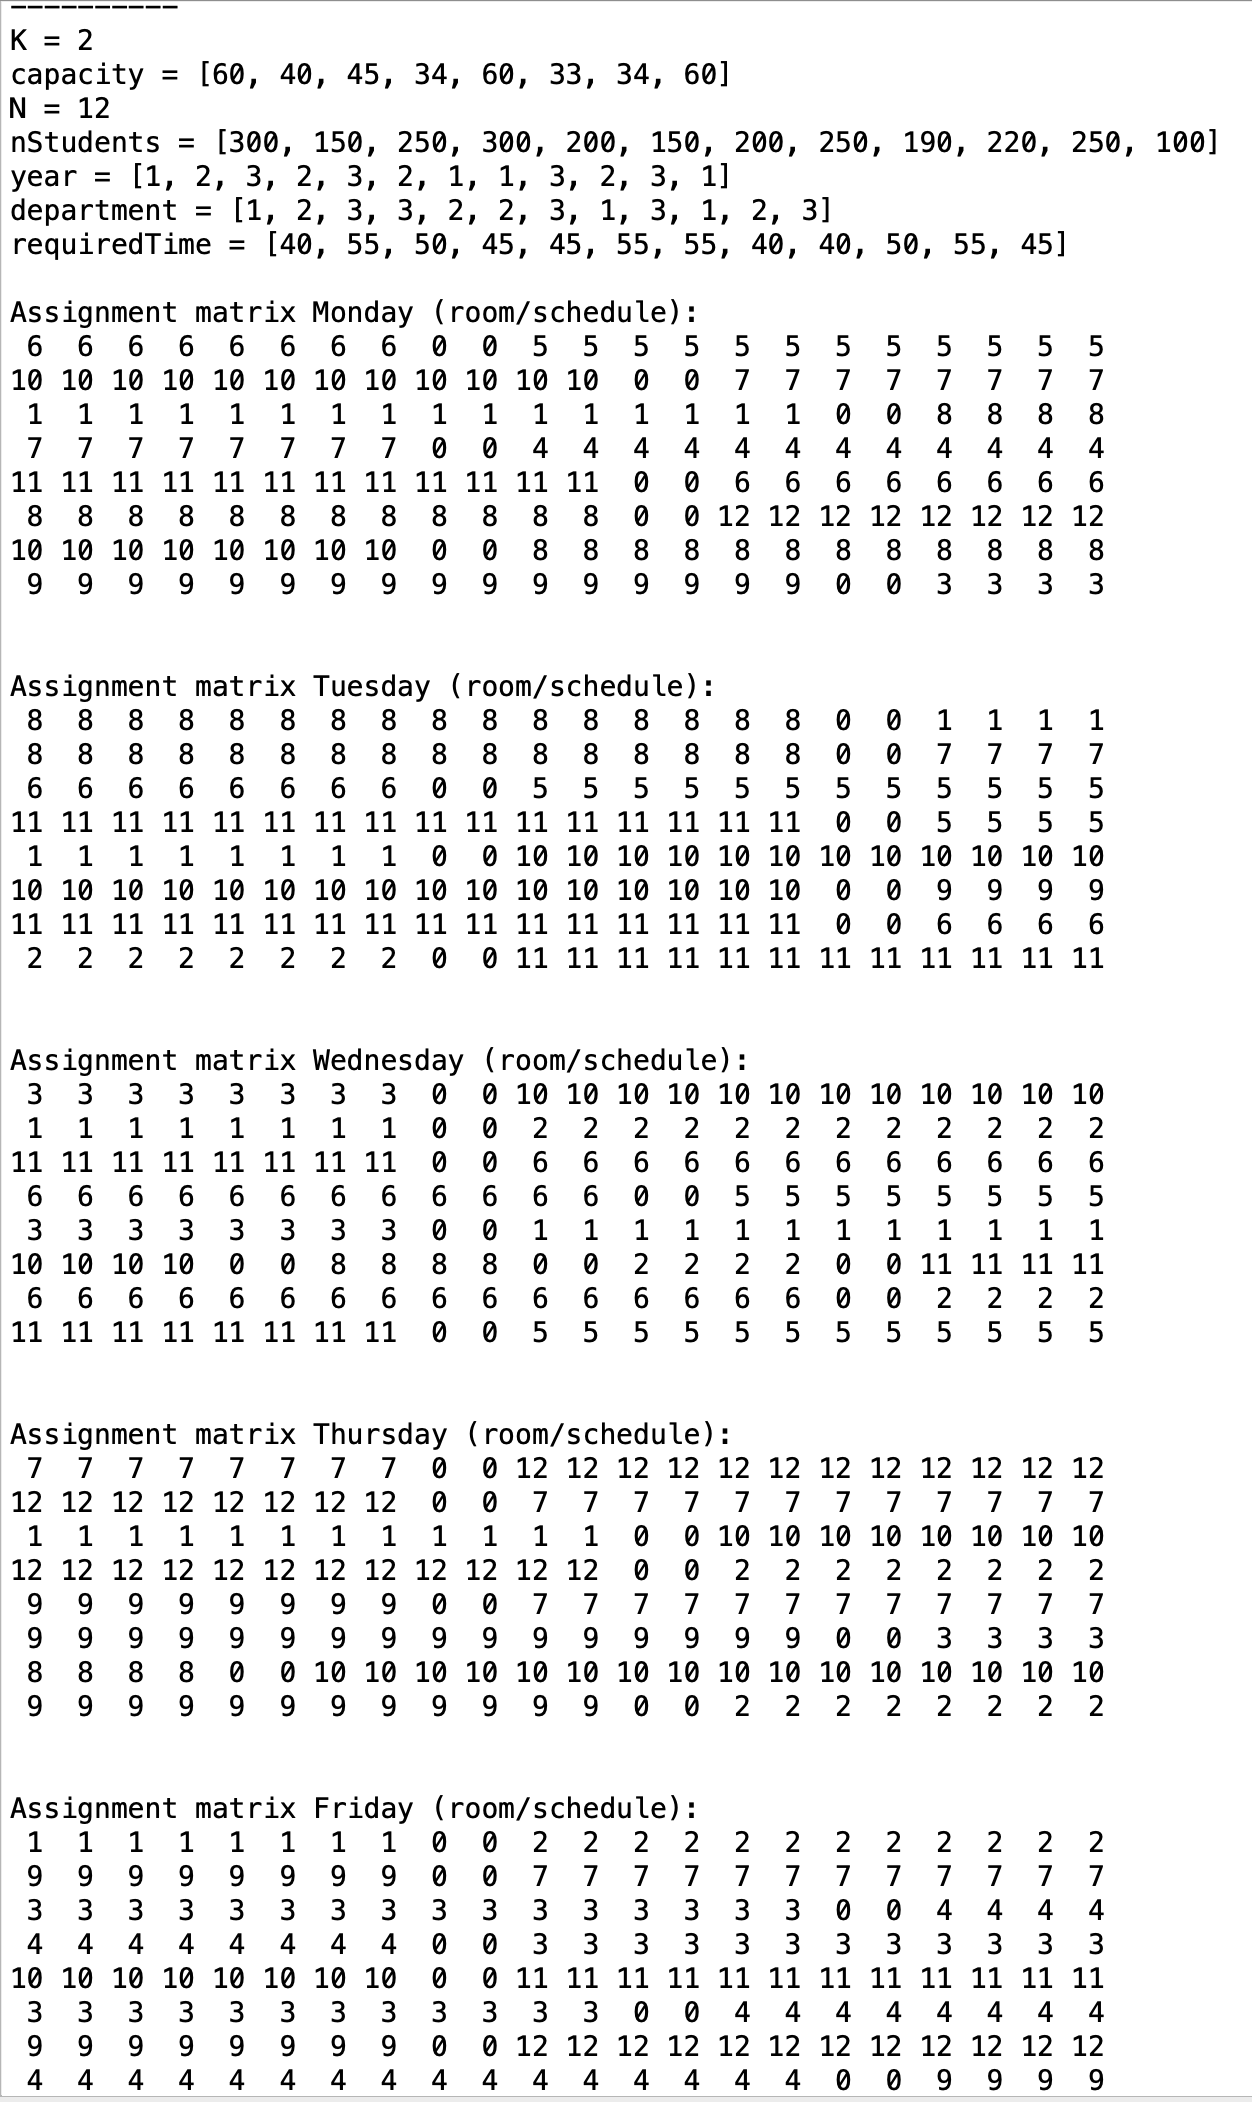
\includegraphics[scale=0.5]{Output_MiniZinc}
\caption{Output del modello MiniZinc sul file \texttt{data1.mzn}}
\label{esempio}
\end{figure}

\chapter{La soluzione in ASP}
La soluzione in ASP è quella che più ha dato problemi nella fase implementativa, i problemi principali sono sorti nell'utilizzo degli aggregati, in particolare nell'utilizzo di \texttt{\#sum}. Andando a vedere la documentazione di \texttt{clingo} \cite{DBLP:journals/corr/GebserKKS14}, la causa di tali problemi è stata individuata e consiste nel modo in cui avviene la valutazione di predicati nel quale il risultato di un aggregato viene prima assegnato ad una variabile (e/o ad un predicato) e poi confrontato con operatori relazionali. Si consideri il seguente codice ASP:

\begin{lstlisting}[style=aspstyle]
{a; b; c}.
:- #sum{1 : a; 2 : b; 3 : c} = N, N > 3.
\end{lstlisting}
questo codice durante la valutazione dà luogo a tre vincoli di integrità:
\begin{lstlisting}[style=aspstyle]
#sum{1 : a; 2 : b; 3 : c} = 4.
#sum{1 : a; 2 : b; 3 : c} = 5.
#sum{1 : a; 2 : b; 3 : c} = 6.
\end{lstlisting}
tale comportamento può essere evitato confrontando direttamente il valore di \texttt{\#sum} invece di assegnarlo prima alla variabile \texttt{N}, tuttavia non sempre ciò è fattibile.\\
Si consideri il vincolo sul bilanciamento delle percentuali di ore insoddisfatte tra i dipartimenti, tale vincolo richiede necessariamente di calcolare ed assegnare a delle variabili il tempo totale di lezione in presenza richiesto da ogni dipartimento ed il tempo totale che gli viene effettivamente assegnato; tali valori vengono confrontati tra loro in quanto al fine del vincolo in questione vengono considerati unicamente i dipartimenti per cui il tempo di lezione in presenza che gli viene assegnato è minore del tempo da loro richiesto, infine presi due dipartimenti diversi deve anche essere calcolata la differenza tra le percentuali di soddisfazione (eq. insoddisfazione) delle ore richieste tra i due dipartimenti e tale differenza deve essere verificata essere minore o uguale al $10\%$. \\
Per le stesse motivazioni è stato evitato di considerare nella funzione di costo la percentuale di studenti che non riesce ad avere lezioni in presenza, in quanto tale calcolo farebbe esplodere il tempo di esecuzione del modello.

\section{Implementazione del vincolo di regolarità}
Il vincolo di regolarità è stato implementato attraverso una definizione esaustiva e mutuale di ciò che consideriamo come slot di lezione valido e ciò che consideriamo come slot di sanificazione valido. Le definizioni di \texttt{lectureSlot/4} e \texttt{sanificationSlot/3} derivano direttamente dalla definizione del vincolo di regolarità descritto nel capitolo \ref{reg}.
Una volta definiti \texttt{lectureSlot/4} e \texttt{sanificationSlot/3} l'unico vincolo inserito nel modello a riguardo è che si richiede che al primo istante di ogni giornata, in ogni aula, sia pianificato uno slot di lezione; data la natura mutuale che caratterizza la definizione di \texttt{lectureSlot/4} e \texttt{sanificationSlot/3} segue la corretta implementazione del vincolo di regolarità.

\section{La funzione di costo}
La funzione di costo descritta in \ref{costo} è stata implementata utilizzando la sintassi offerta dal linguaggio per specificare i vincoli deboli, le priorità dei tre valori interessati sono specificate direttamente all'interno della specifica dei singoli vincoli deboli.
In questo caso viene considerato l'ordine lessicografico delle tuple $(Z, S, K) \in \mathbb{N} \times \mathbb{N} \times \mathbb{N}$ dove $Z$ è il numero di coorti a cui non è assegnato almeno il numero di ore da loro richieste, $S$ è la somma delle percentuali di ore di lezione in presenza mancanti rispetto a quelle richieste tra i vari dipartimenti e $K$ è il numero di unità di tempo assegnate alle sanificazioni.

\section{Il codice}
Viene qui riportato il codice della soluzione in ASP, le parti relative alla generazione dell'output sono omesse.

\lstinputlisting[style=aspstyle, lastline=111]{../asp/model.lp}

\chapter{Esperimenti}
Per testare i due modelli è stata progettata una suite di tests generati prevalentemente in modo casuale. 
Sono stati utilizzati rispettivamente \texttt{clingo} per ASP e \texttt{GeCode} per MiniZinc.
Sono state generate $100$ istanze totali su cui entrambi i modelli sono stati lanciati per $5$ minuti sfruttando $4$ thread su ogni istanza e da cui sono stati ricavati i $3$ parametri coinvolti per il calcolo della funzione di costo descritta in \ref{costo}.\\
Delle $100$ istanze generate, per $50$ di esse $K$, il numero di aule per ognuno dei $4$ gruppi di aule è stato fissato a $1$ (per un totale di $4$ aule), e per le rimanenti $50$ istanze è stato fissato a $2$ (per un totale di $8$ aule). La scelta di limitare $K$ ad un valore massimo pari a $2$ è derivato dai test svolti durante l'implementazione dei due modelli; in particolare a limitare il valore di $K$ sono stati i risultati forniti dal modello ASP che per valori più grandi di $K$ non ha ottenuto risultati soddisfacenti.\\
Il valore di $N$, il numero di coorti, è generato casualmente tra $G*K$ (il numero di aule) e $15$, in questo caso è stato il modello MiniZinc a fornire l'indicazione per il valore massimo di $N$, in quanto con valori più alti di $15$ il modello incominciava ad ottenere risultati insoddisfacenti.
Il numero di dipartimenti diversi, $D$, è stato fissato a $3$ per tutte le istanze, questa scelta è dettata dal fatto che il vincolo di bilanciamento tra le percentuali di insoddisfazione dei diversi dipartimenti è quello più oneroso dal punto di vista computazionale, soprattutto per l'implementazione ASP.\\
Gli altri parametri, quali le capacità delle aule, il numero di studenti delle coorti, l'anno delle coorti, il dipartimento delle coorti, ed il tempo richiesto da ogni coorte sono generati casualmente all'interno del range specificato nelle codifiche ASP e MiniZinc.

Nelle tabelle \ref{res1}, \ref{res2}, \ref{res3}, \ref{res4} sono riportati i risultati dell'esecuzione dei due modelli sulle $100$ istanze generate. I valori riportati sono i parametri $K$ ed $N$, $nUS$ che riporta il numero di coorti alle quali non sono state assegnate le ore di lezione in presenza da loro richieste, $avg(US)$ (resp. $max(US)$) ossia il valore medio della percentuale di insoddisfazione tra i dipartimenti (resp. il valore massimo) e $nSan$ che indica il numero di unità di tempo assegnate alle sanificazioni.
Le celle vuote indicano che il rispettivo modello non ha trovato nessuna soluzione valida.

\section{Commenti sui risultati degli esperimenti}
Dai risultati ottenuti emerge che il modello ASP è più efficace nel trovare una soluzione valida al problema di quanto non lo sia il modello MiniZinc. Tuttavia, durante la fase implementativa era emerso che il modello MiniZinc lavora meglio su valori di $K$ più alti e peggio su valori di $N$ più alti, un ipotesi per spiegare questo comportamento riguarda l'automa utilizzato per riconoscere il vincolo di regolarità, che ricordiamo ha un numero di stati che aumenta linearmente all'aumentare di $N$. Dall'altra parte invece, il modello ASP soffre maggiormente all'aumentare di $K$ e conseguentemente del numero di aule, dato che un grosso collo di bottiglia di tale implementazione pare essere il vincolo riguardante le coorti al primo anno i cui studenti devono avere almeno una lezione in presenza a settimana.\\
Va anche detto che considerare solamente $K$ ed $N$ come parametri porta ad una grossa mancanza di informazione, dato che non stiamo considerando quanti studenti ha ogni coorte, i dipartimenti a cui sono assegnate, il numero di ore che richiedono e quante sono al primo anno.\\
Un'altra osservazione riguarda la qualità dei risultati, per istanze dove il numero di coorti è decisamente maggiore del numero di aule \ref{res2} il modello ASP sembrerebbe fornire generalmente risultati migliori del modello MiniZinc riuscendo sempre ad ottenere un numero di coorti insoddisfatte minore o uguale al corrispettivo ottenuto dal modello MiniZinc, sembrerebbe invece che il modello MiniZinc si concentri troppo sul cercare di minimizzare il numero di sanificazioni. Questo comportamento può essere causato dal diverso modo utilizzato dai due modelli per valutare la funzione di costo, ricordando che i coefficienti utilizzati nella funzione di costo in MiniZinc sono stati scelti arbitrariamente.\\
Per istanze dove il numero di coorti è simile al numero di aule \ref{res1} \ref{res3} \ref{res4} è il modello MiniZinc a fornire risultati migliori, riuscendo nella maggior parte dei casi a soddisfare le richieste di tutte le coorti.

\chapter{Considerazioni e conclusioni}
In questo report abbiamo mostrato due modelli per risolvere un problema di grande attualità quale è quello della generazione degli orari universitari considerando le necessità comportate da una pandemia in corso, i due modelli hanno prodotto risultati soddisfacenti riuscendo a generare effettivamente degli orari per le lezioni validi rispetto alle nostre specifiche sulla maggior parte delle istanze considerate.\\
Purtroppo non è stato possibile raggiungere l'ottimo globale per nessuna delle istanze considerate, e dunque non abbiamo dati empirici per provare ad inferire la complessità del problema trattato, tuttavia è risaputo che il problema sottostante al problema considerato è $NP$-completo in quasi ogni sua variante. \cite{DBLP:journals/air/Schaerf99}\\
Certamente i due modelli non sono privi di problemi, primo su tutti il fatto che non vengono considerate per le coorti non al primo anno quanti studenti non riescono ad avere lezioni in presenza.
I modelli potrebbero essere resi più efficienti rilassando qualche vincolo, ad esempio il vincolo di regolarità, e ancora meglio, potrebbero essere resi più efficienti assegnando di default qualche coorte a delle aule predefinite, per esempio all'inizio del primo giorno della settimana, in modo da tagliare lo spazio di ricerca considerato.


\chapter{Tabelle dei risultati}
\begin{table}[h]
\begin{tabular}{ll|lll|lll}
\multicolumn{2}{l|}{Param} & \multicolumn{3}{l|}{ASP} & \multicolumn{3}{l}{MZN} \\ \hline
K             & N              & nUS    & avg(US)   & nSan     & nUS      & max(US)     & nSan     \\ \hline
1           & 4            & 0    & 0         & 40    & 0    & 0         & 44   \\
1           & 4            & 0    & 0         & 40    & 0    & 0         & 44   \\
1           & 4            & 0    & 0         & 40    & 0    & 0         & 44   \\
1           & 4            & 0    & 0         & 40    & 0    & 0         & 44   \\
1           & 4            & 0    & 0         & 40    & 0    & 0         & 40   \\
1           & 4            & 0    & 0         & 40    & 0    & 0         & 44   \\
1           & 5            & 0    & 0         & 40    & 0    & 0         & 44   \\
1           & 5            & 0    & 0         & 40    & 0    & 0         & 40   \\
1           & 5            & 0    & 0         & 40    & 0    & 0         & 40   \\
1           & 6            & 0    & 0         & 40    & 0    & 0         & 44   \\
1           & 6            & 0    & 0         & 40    & 0    & 0         & 40   \\
1           & 6            & 0    & 0         & 68    & 0    & 0         & 40   \\
1           & 6            & 0    & 0         & 40    & 0    & 0         & 40   \\
1           & 6            & 0    & 0         & 40    & 0    & 0         & 40   \\
1           & 7            & 1    & 18        & 44    & 0    & 0         & 40   \\
1           & 7            & 0    & 0         & 44    & 0    & 0         & 40   \\
1           & 7            & 0    & 0         & 56    & 0    & 0         & 40   \\
1           & 7            & 0    & 0         & 40    & 0    & 0         & 40   \\
1           & 8            & 2    & 58        & 92    & 5    & 14        & 40   \\
1           & 8            & 2    & 67        & 60    & 5    & 9         & 40   \\
1           & 8            & 2    & 33        & 64    & 3    & 2         & 40   \\
1           & 9            & 2    & 71        & 52    & 7    & 20        & 40   \\
1           & 9            & 3    & 47        & 60    & 7    & 24        & 40   \\
1           & 9            & 4    & 75        & 60    & 8    & 37        & 40   \\
1           & 10           & 6    & 51        & 76    & 8    & 40        & 40   \\ \hline
\end{tabular}
\caption{Risultati dell'esecuzione dei due modelli sulle istanze di test da (1-25).}
\label{res1}
\end{table}

\begin{table}[]
\begin{tabular}{ll|lll|lll}
\multicolumn{2}{l|}{Parametri} & \multicolumn{3}{l|}{ASP} & \multicolumn{3}{l}{MiniZinc} \\ \hline
K             & N              & nUS    & avg(US)   & nSan     & nUS      & max(US)     & nSan     \\ \hline
1           & 10           & 6    & 40        & 52    & 9    & 38        & 40   \\
1           & 10           & 6    & 47        & 40    & 9    & 33        & 40   \\
1           & 10           & 5    & 70        & 64    & 9    & 32        & 40   \\
1           & 11           & 7    & 46        & 44    & 9    & 52        & 40   \\
1           & 11           & 5    & 63        & 48    & 8    & 53        & 40   \\
1           & 11           & 8    & 24        & 44    & 10   & 44        & 40   \\
1           & 11           & 7    & 64        & 60    & 10   & 47        & 40   \\
1           & 11           & 8    & 59        & 40    & 9    & 55        & 40   \\
1           & 11           & 7    & 54        & 72    & 9    & 51        & 40   \\
1           & 12           & 8    & 58        & 72    & 10   & 62        & 40   \\
1           & 12           & 8    & 52        & 44    & 11   & 56        & 40   \\
1           & 12           & 8    & 53        & 68    & 10   & 51        & 40   \\
1           & 12           & 9    & 21        & 52    & 11   & 52        & 40   \\
1           & 12           & 8    & 64        & 64    & 11   & 52        & 40   \\
1           & 12           & 8    & 70        & 72    & 11   & 53        & 40   \\
1           & 14           & 11   & 61        & 72    & 13   & 69        & 40   \\
1           & 14           & 11   & 63        & 48    & 12   & 69        & 40   \\
1           & 14           & 10   & 33        & 60    & 13   & 70        & 40   \\
1           & 14           & 12   & 20        & 44    & 12   & 71        & 40   \\
1           & 14           & 11   & 59        & 72    & 13   & 65        & 40   \\
1           & 15           & 11   & 29        & 60    & 14   & 63        & 40   \\
1           & 15           & 12   & 26        & 44    & 14   & 67        & 40   \\
1           & 15           & 11   & 29        & 52    & 14   & 71        & 40   \\
1           & 15           & 12   & 45        & 44    & 14   & 66        & 40   \\
1           & 15           & 13   & 16        & 44    & 13   & 72        & 40   \\ \hline
\end{tabular}
\caption{Risultati dell'esecuzione dei due modelli sulle istanze di test da (26-50).}
\label{res2}
\end{table}

\begin{table}[]
\begin{tabular}{ll|lll|lll}
\multicolumn{2}{l|}{Parametri} & \multicolumn{3}{l|}{ASP} & \multicolumn{3}{l}{MiniZinc} \\ \hline
K             & N              & nUS    & avg(US)   & nSan     & nUS      & max(US)     & nSan     \\ \hline
2           & 8            & 0    & 0         & 92    & 0    & 0         & 80   \\
2           & 8            & 0    & 0         & 92    & 0    & 0         & 84   \\
2           & 8            & 0    & 0         & 100   & 0    & 0         & 84   \\
2           & 8            & 0    & 0         & 100   & 0    & 0         & 84   \\
2           & 8            & 0    & 0         & 116   & 0    & 0         & 80   \\
2           & 8            & 1    & 50        & 100   & 0    & 0         & 80   \\
2           & 8            & 0    & 0         & 84    & 0    & 0         & 84   \\
2           & 8            & 0    & 0         & 108   & 0    & 0         & 84   \\
2           & 9            & 0    & 0         & 128   & 0    & 0         & 88   \\
2           & 9            & 0    & 0         & 116   & 0    & 0         & 88   \\
2           & 9            & 0    & 0         & 120   & 0    & 0         & 84   \\
2           & 9            & 0    & 0         & 100   & 0    & 0         & 84   \\
2           & 9            & 2    & 4         & 100   & 0    & 0         & 84   \\
2           & 9            & 1    & 71        & 96    & 0    & 0         & 80   \\
2           & 9            & 0    & 0         & 88    & 0    & 0         & 84   \\
2           & 10           & 0    & 0         & 100   & 0    & 0         & 84   \\
2           & 10           & 4    & 16        & 104   & 0    & 0         & 80   \\
2           & 10           & 3    & 44        & 100   & 0    & 0         & 84   \\
2           & 10           & 1    & 22        & 112   & 0    & 0         & 84   \\
2           & 10           & 0    & 0         & 84    & 0    & 0         & 92   \\
2           & 10           & 3    & 50        & 120   & 0    & 0         & 80   \\
2           & 10           & 3    & 35        & 92    & 0    & 0         & 84   \\
2           & 10           & 2    & 12        & 100   & 0    & 0         & 88   \\
2           & 11           & 3    & 51        & 108   & 0    & 0         & 92   \\
2           & 11           & 2    & 15        & 108   & 0    & 0         & 80   \\ \hline
\end{tabular}
\caption{Risultati dell'esecuzione dei due modelli sulle istanze di test da (51-75).}
\label{res3}
\end{table}

\begin{table}[]
\begin{tabular}{ll|lll|lll}
\multicolumn{2}{l|}{Parametri} & \multicolumn{3}{l|}{ASP} & \multicolumn{3}{l}{MiniZinc} \\ \hline
K             & N              & nUS    & avg(US)   & nSan     & nUS      & max(US)     & nSan     \\ \hline
2           & 11           & 4    & 39        & 104   & 0    & 0         & 84   \\
2           & 11           & 1    & 22        & 112   & 0    & 0         & 84   \\
2           & 11           & 2    & 28        & 112   & 0    & 0         & 84   \\
2           & 11           & 3    & 42        & 116   & 0    & 0         & 84   \\
2           & 11           & 4    & 55        & 100   & 0    & 0         & 88   \\
2           & 11           & 1    & 52        & 128   & 0    & 0         & 88   \\
2           & 11           & 1    & 21        & 100   & 0    & 0         & 84   \\
2           & 11           & 3    & 49        & 88    & 4    & 8         & 84   \\
2           & 11           & 1    & 34        & 116   & 0    & 0         & 84   \\
2           & 12           & 6    & 29        & 100   & 0    & 0         & 84   \\
2           & 12           & 5    & 36        & 104   & 0    & 0         & 80   \\
2           & 12           & 3    & 20        & 92    & 5    & 12        & 88   \\
2           & 12           & 3    & 37        & 100   & 6    & 14        & 84   \\
2           & 12           & 6    & 51        & 84    & 4    & 7         & 84   \\
2           & 13           & 4    & 40        & 112   & 7    & 6         & 84   \\
2           & 13           & 7    & 23        & 92    &      &           &      \\
2           & 13           & 6    & 63        & 192   & 2    & 5         & 80   \\
2           & 14           & 9    & 44        & 128   &      &           &      \\
2           & 14           & 7    & 43        & 112   &      &           &      \\
2           & 15           & 8    & 35        & 108   &      &           &      \\
2           & 15           & 6    & 34        & 92    & 5    & 10        & 80   \\
2           & 15           & 8    & 47        & 120   &      &           &      \\
2           & 15           & 11   & 46        & 88    &      &           &      \\
2           & 15           & 9    & 31        & 100   &      &           &      \\
2           & 15           &      &           &       &      &           &     \\ \hline
\end{tabular}
\caption{Risultati dell'esecuzione dei due modelli sulle istanze di test (76-100).}
\label{res4}
\end{table}

\pagebreak

% Adding a bibliography if citations are used in the report
% Un/Comment the following line to customize the Bibliography title
\renewcommand{\bibname}{References}
\bibliographystyle{plain}
\bibliography{ref}

% Uncomment the following two lines to remvoe the cc license
\vspace*{\fill}
{\hypersetup{urlcolor=black}{\scriptsize \doclicenseThis}}
% Adds reference to the Bibliography in the ToC
\addcontentsline{toc}{chapter}{\bibname}

\pagebreak


\end{document}